\begin{abstract}
This document contains a problem based on conic problems.
\end{abstract}

Download the python codes from 
%
\begin{lstlisting}
https://github.com/sahilsin/MatrixTheory/tree/master/Assignment4/codes
\end{lstlisting}
%
\section{PROBLEM}
Trace the parabolas $144x^2-120xy+25y^2+619x-272y+663=0$, and find its focus. 

\section{SOLUTION}

\begin{align}
    144x^2-120xy+25y^2+619x-272y+663=0
\\
    (12x-5y)^2=272y-619x-663 
\end{align}

Introducing a variable $\lambda$

\begin{align}
    (12x-5y+\lambda)^2=
\\
    272y-619x-663-10\lambda y+24\lambda x+\lambda ^2
\\
    (12x-5y+\lambda)^2=
\\
    (272-10\lambda)y-(619-24\lambda)x+\lambda^2-663
\end{align}

\begin{align}
    12x-5y+\lambda=0
\\
    (272-10\lambda)y-(619-24\lambda)x+\lambda^2-663=0
\end{align}

For $\lambda$ we assume both lines to be perpendicular

\begin{multline}
\\
    m=-\cfrac{12}{-5}=\cfrac{12}{5}
\\
    m'=-\cfrac{-(619-24\lambda)}{272-10\lambda}
\\
    m \times m'= -1
\\
    \cfrac{12}{5} \times \cfrac{-(619-24\lambda)}{272-10\lambda}=-1
\\
    7428-288\lambda=50\lambda-1360
\\
    \implies \lambda = 26
\\
    (12x-5y+26)^2
\\
    =(272-10\times26)y-(619-24\times26)x
\\
    +(26)^2-663
\\
    \implies (12x-5y+26)^2=5x+12y+13
\\
    \myvec{\cfrac{12x-5y+26}{13}}^2=\cfrac{1}{13}\myvec{\cfrac{5x-12y+13}{13}}
\\
    Y=\cfrac{12x-5y+26}{13}
\\
    X=\cfrac{5x-12y+13}{13}
\\
    Y^2=\cfrac{1}{13}X
\end{multline}

Comparing with equation of parabola $y^2=4ax$:

\begin{align}
    4a=\cfrac{1}{13}
\\
    a=\cfrac{1}{52}
\end{align}

\begin{figure}[!ht]
    \centering
    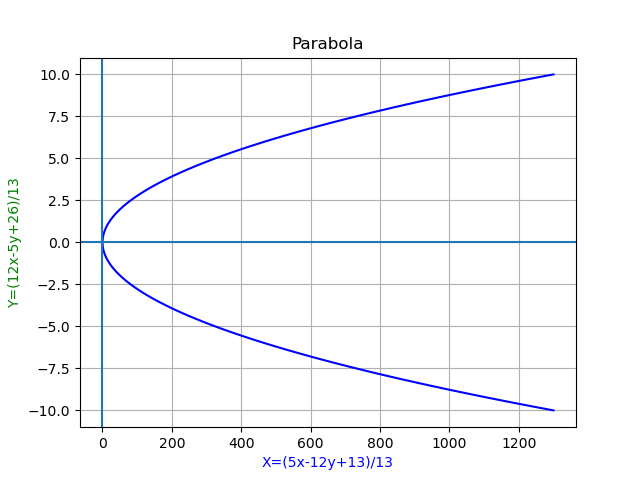
\includegraphics[width=\columnwidth]{./figs/parabola}
\caption{Traced parabola}
\label{parabola}
\end{figure}

The focus of the parabola is obtained by solving $X-a=0$ and $Y=0$.
\begin{align}
    \cfrac{5x-12y+13}{13}-a=0
\\
    \cfrac{5x-12y+13}{13}-\cfrac{1}{52}=0
\\
    20x+48y+51=0\label{eq : 1}
\end{align}

\begin{align}
    \cfrac{12x-5y+26}{13}=0
\\
    12x-5y+26=0 \label{eq : 2}
\end{align} 
 
Solving \ref{eq : 1} and \ref{eq : 2} we get :

\begin{align}
    x=-\cfrac{1503}{676}
\\
    y=-\cfrac{23}{169}
\end{align}

The focus is :
\begin{align}
    \myvec{-\cfrac{1503}{676},-\cfrac{23}{169}}
\end{align}



